% --------------------------------------------------------------
% This is all preamble stuff that you don't have to worry about.
% Head down to where it says "Start here"
% --------------------------------------------------------------

\documentclass[11pt]{article}
\usepackage[margin=0.7in]{geometry}
\usepackage{amsmath,amsthm,amssymb}
%\usepackage{multicol}
\usepackage{graphicx}
%\usepackage{fixltx2e}
%\usepackage{amsmath}

\usepackage{tikz}
\usepackage{pgfplots}
\usepackage{fourier}
\usepackage[inline]{enumitem}



\title{\Large Department of Electronic and Telecommunication Engineering\\University of Moratuwa\\Sri Lanka\\{\LARGE \bf \textsc{EN1060 Signals and Systems: Tutorial 01}}}

\date{\vspace{-0.2in}\today}


\newcommand{\N}{\mathbb{N}}
\newcommand{\Z}{\mathbb{Z}}

\begin{document}



\maketitle
\noindent \tikz \draw (0,0) -- (\textwidth,0);

\begin{enumerate}
\item A continuous time signal is given in Figure 1. Sketch and label the following signals.\par
\begin{enumerate*}
    \item $x(t-2)$
    \item $x(t+1)$
    \item $x(-t+1)$
    \item $x(3t/2)$
    \item $x(t/3)$
\end{enumerate*}


\begin{figure}[h]
    \centering
        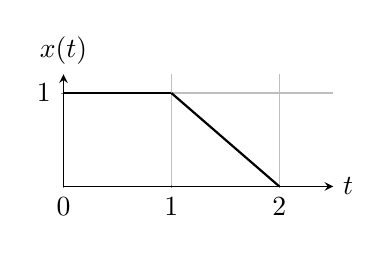
\begin{tikzpicture}
	\begin{axis}[
		xscale = 0.5,
		yscale = 0.25,
		xmin= 0, xmax = 2.5,
		ymin= 0, ymax = 1.2,
		axis x line=bottom, 
		axis y line=center,
		xtick = {0,1,2, 3},
		ytick = {1},
		xlabel=$t$, xlabel style={at={(ticklabel* cs:1)}, anchor= west},
		ylabel=$x(t)$, ylabel style={at={(ticklabel* cs:1)}, anchor=south},
		grid=both,
		]
		\addplot[domain=0:1, thick] (\x, 1);
		\addplot[domain=1:2, thick] (\x, 2-\x);
	\end{axis}
\end{tikzpicture}
\caption{}
\end{figure}

\item A discrete time signal is shown in Figure 2. Sketch and label each of the following signals.\par
\begin{enumerate*}
    \item $x[n+1]$
    \item $x[2n]$
    \item $x[-n]$
    \item $x[-n +2]$
    \item $x[-2n+1]$
\end{enumerate*}


\begin{figure}[h]
    \centering
    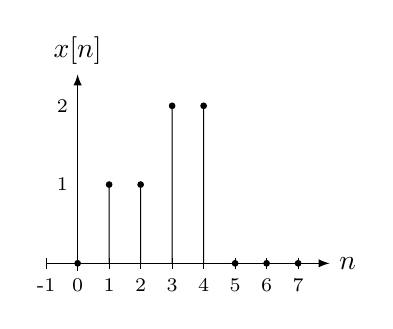
\begin{tikzpicture}
    \draw[-latex] (-1*0.4,0) -- (8*0.4,0) node[anchor=west] {$n$};
    \draw[-latex] (0, -0.1) -- ++(0,2.5) node[anchor=south] {$x[n]$};
    \foreach \x in {0}
        {
            \draw[fill=black] (\x*0.4, 0) circle (1pt);
        }
    \foreach \x in {1,2}
        {
            \draw[fill=black] (\x*0.4, 0)  -- ++(0,1) circle (1pt);
        }
    \foreach \x in {3,4}
        {
            \draw[fill=black] (\x*0.4, 0)  -- ++(0,2) circle (1pt);
        }        
        
    \foreach \x in {5,6,7}
        {
            \draw[fill=black] (\x*0.4, 0) circle (1pt);
        }        
    \foreach \x in {-1, 0, ..., 7}
    {
        \draw (\x*0.4, 2pt) -- ++(0, -4pt) node[anchor=north]{\scriptsize \x};
    }
    \foreach \y in {1,2}
    {    
    	\node at (0,\y) [anchor=east] {\scriptsize \y};
    }
\end{tikzpicture}
\caption{}
\end{figure}

\item Find the even and odd parts of the $x(t)$ signal given in Figure \ref{fig03}.
\begin{figure}[h]
    \centering
    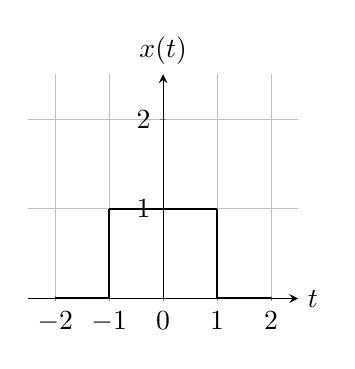
\begin{tikzpicture}
	\begin{axis}[
		xscale = 0.5,
		yscale = 0.5,
		xmin= -2.5, xmax = 2.5,
		ymin= 0, ymax = 2.5,
		axis x line=bottom,
		axis y line=center,
		xtick = {-2,-1,0,1,2},
		ytick = {1, 2},
		xlabel=$t$, xlabel style={at={(ticklabel* cs:1)}, anchor= west},
		ylabel=$x(t)$, ylabel style={at={(ticklabel* cs:1)}, anchor=south},
		grid=both,
		]
		\addplot[domain=-1:1, thick] (\x, 1);
		\addplot[domain=-2:-1, thick] (\x, 0);
        \addplot[domain=1:2, thick] (\x, 0);
        \draw[thick] (axis cs:-1,0) -- (axis cs:-1,1);
        \draw[thick] (axis cs:1,0) -- (axis cs:1,1);
        \end{axis}
\end{tikzpicture}
\caption{}
\label{fig03}
\end{figure}

\item Using the discrete time signals $x_1[n]$ and $x_2[n]$ shown in Figure 4, represent each of the following signals by a graph.\par
\begin{enumerate*}
    \item $y[n] = x_1[n]+ x_2[n]$
    \item $y[n] = 2x_1[n]$
    \item $y[n] = x_1[n]x_2[n]$
\end{enumerate*}

\begin{figure}[h]
    \centering
    \begin{tikzpicture}
	\begin{scope}
	    \draw[-latex] (-3*0.4,0) -- (6*0.4,0) node[anchor=west] {$n$};
	    \draw[-latex] (0, -0.1) -- ++(0,3.5) node[anchor=south] {$x_1[n]$};
	    \foreach \x/\y in {-2/0, -1/0, 0/0, 1/0, 2/2, 3/0, 4/0}
	        {
	            \draw[fill=black] (\x*0.4, 0) -- ++(0,\y) circle (1pt);
	        }
	 
	    \foreach \x in {-2, -1, ..., 4}
	    {
	        \draw (\x*0.4, 2pt) -- ++(0, -4pt) node[anchor=north]{\scriptsize \x};
	    }
	    \foreach \y in {1,2}
	    {
	    	\node at (0,\y) [anchor=east] {\scriptsize \y};
	    }
    \end{scope}
    
    	\begin{scope}[xshift=6cm]
	    \draw[-latex] (-4*0.4,0) -- (5*0.4,0) node[anchor=west] {$n$};
	    \draw[-latex] (0, -0.1) -- ++(0,3.5) node[anchor=south] {$y_1[n]$};
	   \foreach \x/\y in {-2/0, -1/0, 0/0, 1/0, 2/1, 3/2, 4/0}
	        {
	            \draw[fill=black] (\x*0.4, 0) -- ++(0,\y) circle (1pt);
	        }
	 
	    \foreach \x in {-2, -1, ..., 4}
	    {
	        \draw (\x*0.4, 2pt) -- ++(0, -4pt) node[anchor=north]{\scriptsize \x};
	    }
	    \foreach \y in {1,2,3}
	    {
	    	\node at (0,\y) [anchor=east] {\scriptsize \y};
	    }
    \end{scope}

\end{tikzpicture}
\caption{}
\label{fig04}
\end{figure}

\item Show that

\begin{equation*}
    \int_{-a}^{a} x(t) dt =
    \begin{cases}
        2 \int_{0}^{a} x(t) dt, & \text{if $x(t)$ is even,} \\
        0, & \text{if $x(t)$ is odd.} \\
    \end{cases}
\end{equation*}


\item Show that the complex exponential signal $x(t)  = e^{j\omega t}$ is periodic and that its fundamental period is $2\pi / \omega$.

\item Show that the complex exponential signal $x[n]  = e^{j\omega n}$ is periodic only if $\omega / 2\pi$ is a rational number.

\item Consider the sinusoidal signal $x(t) = \cos(15t)$.
\begin{enumerate}
    \item Find the value of sampling interval $T$ such than $x[n]$ is a periodic sequence.
    \item Find the fundamental period of $x[n]$ if $T = 0.1\pi$ seconds.
\end{enumerate}


\item Determine whether or not each of the following signals are periodic. If periodic, find the fundamental period.
\begin{enumerate}
    \item $x(t) =2e^{j(t+\pi/4)}$
    \item $x[n] =e^{j(\pi/4)n}$
    \item $x(t) = \cos(t+\pi/4)$
    \item $x(t) = \cos(t) + \sin(\sqrt{2}t)$
    \item $x[n] = \cos^{2}(\pi n/8)$
\end{enumerate}


\item Determine whether the following signals are energy signals, power signals, or neither.\par
    \begin{enumerate*}
        \item $x(t) = e^{-at}u(t), a > 0$
        \item $x(t) = A\cos(\omega t+\theta)$
        \item $x[n] = 3u[n]$
        \item $x[n] = 3e^{j3n}$
    \end{enumerate*}



\end{enumerate}



\end{document} 